\chapter{Аналитическая часть: введение в понятие соревнований по защите информации}
\label{cha:analysis}

\section{История}

Согласно «Словарю русского языка» C. И. Ожегова, соревнования --- форма деятельности (работы, игры), при которой участвующие стремятся превзойти друг друга \cite{Ozhegov89}. По моему мнению, вышеупомянутое стремление есть неотъемлемая часть человеческой природы и один из определяющих факторов развития нашей цивилизации, ведь прогресс в любой сфере деятельности --- это достижение новых, более совершенных результатов в чём бы то ни было.

\Abbrev{ICPC}{International Collegiate Programming Contest ""--- Международная студенческая олимпиада по программированию}

Соревнования естественным образом возникают и в областях, связанных с информационными технологиями. Так, в 1970 году в Техасском университете A\&M были проведены соревнования по спортивному программированию, ныне известные как ICPC\cite{AboutICPC}. Командам участников предлагали решить несколько формально определённых задач на языке программирования «Фортран». Организаторы засекали время и принимали решения на перфокартах: призовые места распределялись согласно времени, которое команда потратила на решение.

На сегодняшний день ICPC — масштабное, уважаемое и значимое соревнование, к победе в котором стремятся сотни тысяч студентов технических вузов по всему миру. Возникли и другие соревнования по спортивному программированию, например, Всероссийская олимпиада школьников по информатике.

Когорта спортивных программистов внесла существенный вклад в развитие науки и техники. Опыт, получаемый во время тренировок и непосредственного участия в соревнованиях, отразился в компьютерных науках (теория алгоритмов, теория оптимизации, численные методы и др.), методиках преподавания связанных с разработкой программного обеспечения дисциплин и проч. В качестве примера можно привести открытую в 2000 году многократным победителем олимпиад по программированию Николаем Дуровым структуру данных, известную как \textit{декартово дерево по неявному ключу}\cite{Durov00} или возникновение в России системы компьютерных школ и сборов, воспитавших не одно поколение талантливых программистов, архитекторов и учёных\cite{Netrusova09}\cite{Kraivanova12}.

По мере распространения компьютерных технологий закономерно всё актуальнее становился вопрос о их безопасности. Возникло понятние кибербезопасности --- совокупности методов и практик защиты от атак злоумышленников для компьютеров, серверов, мобильных устройств, электронных систем, сетей и данных. И в этой сфере появились свои соревнования. Они проходят в формате CTF \textit{(англ. capture the flag --- «захват флага»)}.

\Define{Кибербезопасность}{совокупность методов и практик защиты от атак злоумышленников для компьютеров, серверов, мобильных устройств, электронных систем, сетей и данных}

\Abbrev{CTF}{capture the flag ""--- формат соревнований по защите информации «захват флага»}

Первые в мире соревнования по защите в таком формате, DEF CON CTF, были проведены в США в 1996 году \cite{Defcon}. Они проходили следующим образом. Организаторы предоставили командам участников модельную компьютерную систему --- некий программный сервис, который принимает пользовательские запросы и неким соответствующим образом их обратывающий. В базе данных сервиса хранились т.н. флаги --- текстовые строки определённого формата, на месте которых в реальной, не модельной, ситуации могли бы оказаться критически важные данные: например, номера банковских карт или пароли. Наконец, в системе были предусмотрены определённые уявзимости, с помощью которых. От участников требовалось запустить предоставленный сервис на своём сервере, доступном из общей игровой сети, поддерживать его в работоспособном состоянии, обнаруживая и исправляя в нём уязвимости; а также использовать найденные уязвимости для «захвата» флагов с аналогичных серверов других команд.

Со временем CTF-соревнования стали массовым явлением. Свои мероприятия проводят такие крупные IT-комании, как Meta\cite{FBCTF}, Google\cite{GoogleCTF}, «Яндекс»\cite{YaCTF} и «Лаборатория Касперского»\cite{KasperskyCTF}. За участие в них победителям выплачивают крупные денежные призы, а сами победители, как правило, получают приглашения на работу во многие крупные компании, специализирующиеся на кибербезопасности.

Интерес к CTF-соревнованиям постепенно появился и за пределами США. В апреле 2008 г. команда «Хакердом», на базе Уральского государственного университета им. А. М. Горького, провела открытые межвузовские соревнования по защите информации RuCTF-2008. В игре приняло участие 9 команд со всей России\cite{Hackerdom08}. Сегодня RuCTF --- международные соревнования, в которых принимают участие сильнейшие команды со всей Европы\cite{Hackerdom20}.

Стоит отметить, что, зачастую организаторы соревнований по защите информации выступают в роли игроков --- и наоборот. Например, прежде чем стать организаторами RuCTF и популяризаторами CTF в России, команда «Хакердом» на протяжении многих лет занимала высокие места в глобальных рейтингах\cite{HackerdomRating}.

Сегодня CTF продолжает набирать популярность. Агрегатор мероприятий ctftime.org содержит в себе сведения более чем о 1300 соревнованиях, прошедших с 2011 года \cite{CTFTimeTotal}. Соревнования всё чаще проводятся в формате многодневных конференций, на которых игроки выступают с докладами и активно обмениваются опытом, к таким относятся:
\begin{enumerate}
  \item DEF CON CTF, Лас-Вегас, США;
  \item PHDays Standoff и PHDays CTF, Москва, Россия;
  \item VolgaCTF, Самара, Россия;
  \item RuCTF, Екатеринбург, Россия и др.
\end{enumerate}

Проводятся и образовательные соревнования, нацеленные, не только на студентов и профессионалов в области кибербезопасности, но и на школьников. Важность обучения последних азам защиты информации в теории и практике подтверждается государственным интересом в этой области. В 2017 году министр образования Российской Федерации Ольга Васильева предложила добавить в школьную программу уроки кибербезопасности \cite{RG17}, а с 2018 года по профилю «Информационная безопасность» в формате CTF проводится Олимпиада Национальной технологической инициативы, организации, которая ставит своей целью достижение глобального технологического лидерства России к 2035 году. Автор этой ВКР участвует в разработке и проведении всероссийской школьной олимпиады по защите информации Ugra CTF (см. пункт \ref{cha:analysis:ugractf}).



\section{Правила, принципы и виды}

За 26 лет формат CTF претерпел множество видоизменений и интерпретаций. Общепринята следующая классификация CTF-соревнований:

\begin{enumerate}
  \item \textbf{attack-defense, A/D} \textit{(англ. нападение и защита)};
  \item \textbf{jeopardy} \textit{(англ. название телепередачи, известной в России как «Своя игра»)}.
\end{enumerate}

Эти виды соревнований существенно отличаются правилами, темпом и сложностью игры. Рассмотрим каждый вид отдельно.


\subsection{Attack-defense CTF}

Этот вид соревнований возник первым. К нему относятся, например, все DEF CON CTF, проведённые с 1996 года по настоящее время.

Данное описание носит усреднённый характер ввиду большого числа независимо проводимых мероприятий и высокой вариации их правил относительно друг друга.

Общие положения:
\begin{enumerate}
  \item Соревнования проходят в общей игровой сети (пример структуры такой сети на рис. \ref{fig:ad}). Каждая команда участников имеет в ней собственный сервер, доступный внутри этой сети и называемый \textit{вулнбоксом} \textit{(англ. vulnerable box, дословно «уязвимая коробка»)}.
  \item Участники получают от организаторов набор сервисов — программного обеспечения, способного принимать, хранить и обрабатывать информацию. Он может быть как заранее установлен организаторами на каждый вулнбокс, так и требовать установки и даже поставляться в заведомо нерабочем состоянии, например, сервисы могу содержать ошибки в программном коде, быть сконфигурированны некорректным образом или использовать библиотеки, отсутствующие в комплекте поставки.
  \item Каждый сервис из набора гарантированно содержит одну или несколько уязвимостей, позволяющих получать несанкционированный доступ к информации, им хранимой.
  \item В начале соревнований сеть сконфигурирована таким образом, что каждой команде доступен только собственный вулнбокс. Таким образом командам предоставляется время на изучение сервисов (как правило, один час).
  \item Затем сеть открывается: включается связь между вулнбоксами разных команд, одновременно с этим начинается отсчёт раундов (как правило, один рануд длится одну минуту).
  \item В течение каждого раунда жюри выполняет следующие действия с каждым сервисом на каждом вулнбоксе:
    \begin{enumerate}
      \item пытается воспользоваться им по назначению, проверяя его работоспособность;
      \item записывает секретные данные, называемые флагом;
      \item проверяет доступность и целостность флагов, записанных в предыдущих раундах.
    \end{enumerate}
  \item Поскольку на всех вулнбоксах рабоают идентичные сервисы, и каждый вулнбокс доступен всем участникам, то с момента открытия сети эти уязвимости можно эксплутировать для «захвата» чужих флагов, сдавая эти флаги членам жюри и получая за это очки.
  \item Участникам также допустимо исправлять обнаруживаемые ими уязвимости при условии, что работоспособность сервисов сохраняется.
\end{enumerate}

\begin{figure}
  \centering
  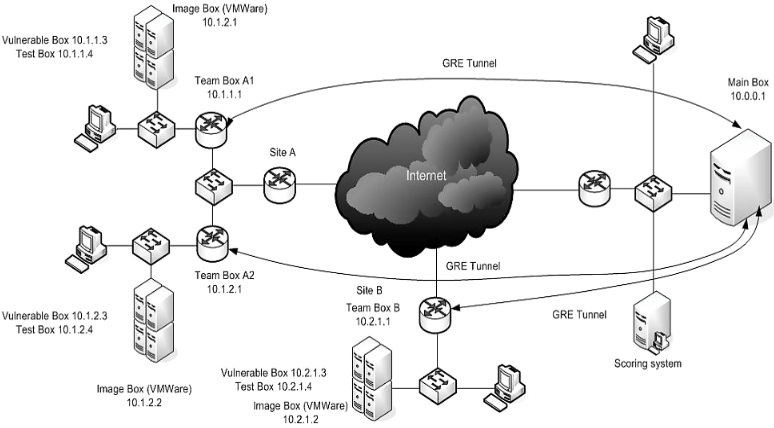
\includegraphics[width=0.9\textwidth]{inc/img/ad}
  \caption{Схема игровой сети UCSB CTF}
  \label{fig:ad}
\end{figure}

Примерная продолжительность такой игры --- от пяти до двенадцати часов. Победителей определяют по сумме баллов, набранных за всю игру.

Соревнования вида attack-defense требовательны к участникам. Для игры базово необходимо обладать следующими навыками и умениями:
\begin{enumerate}
  \item серверное администрирование для настройки и запуска игровых сервисов и конфигурации вулнбоксов;
  \item сетевые технологии для понимания поверхности атак, свзянанных с протоколами, а также для того, чтобы перехватывать трафик (одна из стратегий игры --- наблюдать, как другие команды эксплуатируют уязвимости и как можно быстрее повторять их действия\cite{ReplayAttacks});
  \item быстрое чтение программного кода сервисов, который может быть написан на любом языке программирования: от Python\cite{PythonService} до Haskell\cite{HaskellSerivce} или Bash\cite{BashService};
  \item и т.п.
\end{enumerate}




\subsection{Jeopardy CTF}

Этот вид CTF-соревнований отличается, в первую очередь, более простым набором правил, а также подходом: команды решают задачи, а не атакуют друг друга. Общие положения:

\begin{enumerate}
  \item Участникам предлагается одинаковый набор задач \textit{(англ. challenges)}.
  \item Каждая задача имеет описание, категорию, к которой она относится (см. табл. \ref{tab:categories}), а также стоимость.
  \item Решение каждой задачи подразумевает поиск и сдачу жюри одного флага. За сданный флаг команда получает столько очков, сколько стоило задание.
  \item В конце соревнований подводят итоги. Побеждают команды, первыми набравшие наибольшее число очков.
\end{enumerate}

\begin{figure}
  \centering
  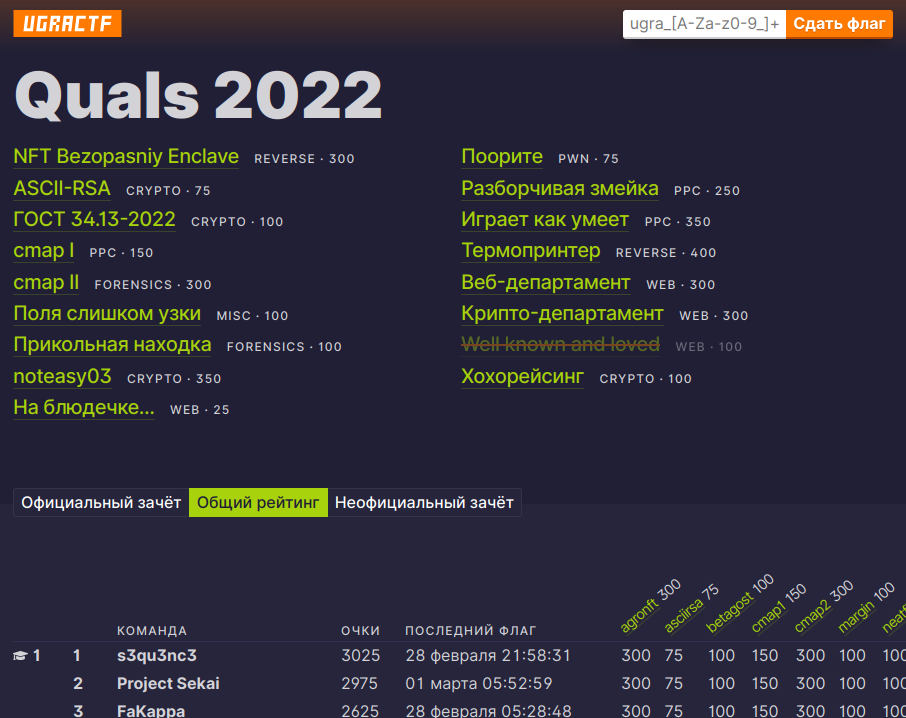
\includegraphics[width=0.5\textwidth]{inc/img/jeopardy}
  \caption{Главная страница игровой системы Ugra CTF}
  \label{fig:jeopardy}
\end{figure}


Своё название данный вид соревнований получил благодаря схожести с форматом телепередачи «Своя игра», в которой игроки выбирают вопросы, сгруппированные по темам и стоимости, с той лишь разницей, что в CTF команды решают задачи асинхронно и не должны видеть решения других команд. Таким образом, соревнования вида jeopardy больше похожи на соревнования по спортивному программированию, где участники получают баллы за верно решённые формально описанные задачи и дисквалифицируются за нечестную игру: списывание или получение иной внешней помощи.

Однако, формат CTF, ввиду своей специфики, даёт больше творческой свободы как составителям задач, так и решающим их людям. В частности, на CTF-соревнованиях --- даже школьных олимпиадах --- разрешается пользоваться интернетом и справочной литературой, поскольку, с одной стороны, решение может требовать от участников способности оперативно разобраться в новой, незнакомой технологии и проэксплуатировать её уязвимости, а с другой, задачи в CTF составляются так, чтобы быть не похожими на уже существующие. Последнему факту способствует важная традиция, принятая в сообществе: как организаторы, так и участники, после окончания соревнований, публикуют в открытом доступе т. н. «райтапы» \textit{(англ. writeup)} --- разборы решений задач. По этой же причине CTF-задачи за редким исключением (в случае закрытых соревнований внутри компаний либо некомпетентности организаторов) не переиспользуются в нескольких соревнованиях.

В отличие от attack-defense, порог входа в соревнования, построенные по принципам jeopardy, существенно ниже. Обычно участникам, чтобы получить доступ к игре, достаточно лишь зарегистрироваться в игровой системе. Из этого не следует, что задачи в jeopardy проще, чем эксплуатация уязвимостей сервисов в attack-defense. Для решения могут пригодиться самые разные умения и навыки. Именно поэтому задачи разделяют на категории, а команды зачастую состоят из специлаистов в непересекающихся областях.

\begin{center}
  \begin{longtable}{|p{0.12\textwidth}|p{0.82\textwidth}|}
    \caption{Некоторые категории CTF-задач}
    \label{tab:categories}
    \\ \hline
    Название & Пояснение
    \\ \hline \endhead
    \texttt{crypto}   & Криптография: задачи о слабых криптоалгоритмах \\
    \texttt{stegano}  & Стеганография: искусство тайной передачи информации \\
    \texttt{osint}    & Разведка по открытым источникам: поиск информации в интернете \\
    \texttt{ppc}      & Программирование: необходимо что-то автоматизировать \\
    \texttt{reverse}  & Реверс-инжиниринг: анализ бинарных файлов или работы программ \\
    \texttt{web}      & Веб-техологии: браузерные и серверные уязвимости \\
    \texttt{network}  & Компьютерные сети \\
    \texttt{admin}    & Администрирование: знание ОС и ПО \\
    \texttt{hardware} & Аппаратные устройства: микроконтроллеры, электротехника и т.п. \\
    \hline
  \end{longtable}
\end{center}

\Abbrev{ОС}{Операционная система}
\Abbrev{ПО}{Программное обеспечение}

Данная работа посвящена разработке среды для проведения соревнований по защите информации именно этого вида.




\section{Соревнования по защите информации Ugra CTF}
\label{cha:analysis:ugractf}

На момент написания данной ВКР автор проходит практику в Югорском научно-исследовательском институте информационных технологий. При поддержке этого института, а также по инициативе Департамента информационных технологий и цифрового развития Ханты-Мансийского автономного округа — Югры, в России с 2016 проводятся соревнования по защите информации Ugra CTF. Традиционно они проводились в два этапа: дистанционный отборочный для всех желающих и очный заключительный (финал) для лучших игроков, проводившийся в столице ХМАО, Ханты-Мансийске. Как правило, оба этапа представляли собой CTF вида jeopardy.

\begin{figure}
  \centering
  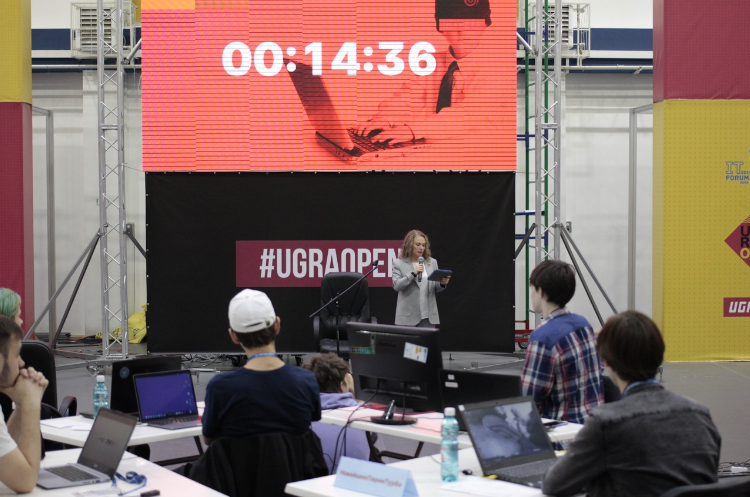
\includegraphics[width=0.6\textwidth]{inc/img/ugractf-19}
  \caption{Открытие Ugra CTF Finals 2019. 10 июня 2020 года, Ханты-Мансийск}
  \label{fig:ugractf-19}
\end{figure}

\Abbrev{ХМАО-Югра}{Ханты-Мансийский автономный округ — Югра}

В 2019–2020 году в состав организаторов вошёл Департамент образования и молодежной политики ХМАО-Югры. Примерно в это же время в России стало наблюдаться снижение числа регулярных CTF-соревнований для школьников. По разным причинам прекратили свою деятельность организаторы соревнований UfoCTF\cite{UfoCTF} и QCTF\cite{QCTF}, основных российских соревнований для новичков. В связи с этим, были внесены изменения в схему проведения соревнований — для школьников с 2021 года проводится отдельный т.н. \textit{распределённо-очный} индивидуальный (вместо командного) заключительный этап по правилам Российского совета олимпиад школьников.

\Abbrev{РСОШ}{Российский совет олимпиад школьников}

Соблюдение правил РСОШ в необходимо для включения соревнований Ugra CTF в государственный перечень школьных олимпиад. Это позволит победителям получать привилегии при поступлении в высшие учебные заведения. Однако, новый формат соревнований означает новые технические и организационные вызовы. Распределённо-очный заключительный этап --- компромисс между:
\begin{enumerate}
  \item полностью дистанционным проведением олимпиады, запрещённым правилами РСОШ ввиду отсутствия возможности контролировать участинков;
  \item полностью очным проведением, когда все участники собираются на единой площадке, полностью контролируемой оргкомитетом.
\end{enumerate}

При таком формате соревнования проходят в разных городах на разных площадках, предоставляемых партнёрами оргкомитета: частными фирмами, образовательными организациями или муниципалитетами. У оргкомитета сохраняется частичный контроль над инфраструктурой --- рабочими станциями участников, которые предоставляются площадками. Каждая площадка также выделяет из своих сотрудников наблюдателей, по совместительству вынужденных выолнять роль системных администраторов, что и вызывает основные сложности.

Соревнования компьютерные: от программного и аппаратного оснащения рабочих станций участников зависит многое. Зачастую требуются привилегированный доступ к системе и специализированные программные инструменты; к тому же дополнительные трудности могут возникать и в свете того, что многие игроки не используют наиболее распространённую в России ОС Windows, предпочитая UNIX-подобные системы как более подходящие для нетривиальных экспериментов, необходимых для решения многих игровых задач.

Настройка инфраструктуры, и контроль за соблюдением порой неочевидных правил требует определённой подготовки наблюдателей, которую оргкомитет по ряду причин не может осуществлять.

Таким образом, существует высокий риск того, что игра пройдёт с нарушениями. Например, согласно правилам РСОШ переговоры участников и получение внешней запрещены, однако, ввиду специфики соревнований пользоваться интернетом школьникам разрешается. Возникает закономерный вопрос: как отличить легитимное использование сети от тщательно замаскированной попытки опубликовать решение и получить помощь третьего лица?

В отборочном этапе 2021 года приняли участие 233 школьника в составе 93 команд. Помимо этого, более 450 команд со всего мира выполняли задания олимпиады в неофициальном зачёте \cite{Ugra21}. В том же этапе, но в 2022 году, приянло участие уже 383 школьника из 159 команд. Из них более 30 прошли в финал.

Для того, чтобы все финалисты смогли принять участие, команде разработки необходимо будет предоставить несколько десятков особым образом настроенных рабочих станций: от Санкт-Петербурга до Владивостока, и обеспечить бесперебойность работы всей инфраструктуры соревнований.



\section{Техническая архитектура соревнований}

Для проведения соревнований Ugra CTF необходима комплексная архитектура, которая позволит решить следующие задачи:

\begin{enumerate}

\item обеспечение решения игровых задач, включая получение условий, приём, валидацию и проверку флагов;
\item

\end{enumerate}

\Abbrev{TCP}{transmission control protocol --- протокол управления передачей}

\subsection{Система, обеспечивающая решение игровых задач}

Соревнования вида jeopardy с самого начала были автоматизированы. Это связано с относительно более тривиальным игровым процессом, чем в соревнованиях вида attack-defense. Обычно участники получают доступ к веб-приложению, которое содержит условия задач, турнирную таблицу и форму для сдачи флага. Его принято называть бордой.

\Define{борда}{\textit{(англ. board, буквально «доска»)} --- программная платформа для получения условий задач и сдачи флагов в CTF-соревнованиях вида jeopardy.}


\subsubsection{Требования к системе}

Борда должна отвечать ряду требований.

\begin{enumerate}

\item
В первую очередь, к таким требованиям можно отнести устойчивость к высоким нагрузкам. В отличие от соревнований вида attack-defense, где нагрузка команды атакуют друг друга (отношение «многие ко многим»), в jeopardy участники взаимодействуют с централизованной игровой инфраструктурой организаторов (отношение «многие к одному»). Отказ в обслуживании со стороны игровой платформы категорически недопустим, поскольку он создаёт неравные условия для игроков: возможна ситуация, когда часть участников успеет получить условие задачи или сдать флаг, в то время как другая --- нет.

Основные операции в платформе должны выполняться быстро и без существенных задержек. Желательно, чтобы система поддерживала многопоточную обработку пользовательских запросов там, где это возможно.

\item
Многопоточность, однако, зачастую приводит к неопределённости параллелизма. Эта неопределённость может послужить причиной ошибок: двойному начислению баллов, списанию некорректной суммы баллов при взятии подсказок или достижению некорректного состояния системы.

\Define{Неопределённость параллелизма}{ошибка проектирования многопоточной системы или приложения, при которой работа системы или приложения зависит от того, в каком порядке выполняются части кода}

\item
Тот факт, что соревнования --- по защите информации, накладывают повышенные требования к безопасности платформы. Не смотря на то, что правилами Ugra CTF запрещены атаки на инфраструктуру, непосредственно не относящуюся к игровым задачам, попытки вывести её из строя всё равно предпринимаются. Система должна быть устойчивой к наиболее распространённым веб-уязвимостям (обработка запросов, контроль пользовательских сессий и проч.), а также вести аудит всех событий для своевременного обнаружения оргкомитетом новых угроз.

\item
Платформа должна позволять обнаружать не только технические угрозы, но и более «человеческие»: пресекать попытки списывания, обмена участников флагами, решения соревнований одним и тем же лицом с нескольких аккаунтов (т.е. мультиаккаунтинг).

\item
Наконец, система должна быть гибкой. CTF --- творческий формат, поэтому структура и принципы могут меняться от игры к игры. Так, отборочный этап Ugra CTF 2019 представлял собой не простой jeopardy, где участникам сразу доступны все задания, а модельный тест на проникновение: сперва игрокам доступна лишь одна точка входа в вымышленную уязвимую систему. По мере «погружения» влубь этой системы открывались новые задания, которые выстраивались в нелинейную древовидную структуру\cite{UgraCTF19Q}.
\end{enumerate}


\subsubsection{Анализ существующих решений}

Существует множество программных продуктов, позволяющих проводить jeopardy -- CTF-соревнования, что называется, «под ключ»: организаторам необходимо лишь собрать участников, разработать задания и загрузить их на готовую платформу, при необходимости изменив некоторые её параметры. К сожалению, автору не удалось обнаружить такой системы, которая удовлетворяла бы всем требованиям \textit{(а)---(д)}, данным выше (табл. \ref{tab:boards}).

\begin{center}
  \begin{longtable}{|p{0.26\textwidth}|p{0.15\textwidth}|p{0.25\textwidth}|c|c|c|c|c|}
    \caption{Сравнительный анализ наиболее популярных готовых jeopardy-платформ}
    \label{tab:boards}
    \\ \hline
    \multirow{2}{*}{Название} & \multirow{2}{*}{Лицензия} & \multirow{2}{*}{Комментарий} & \multicolumn{5}{c|}{Требования} \\ \cline{4-8}
                              &                           &                              & (а) & (б) & (в) & (г) & (д) \\
    \hline \endhead
    ctfd                  & Коммерческая & \small{Непроизводительная}                     & − & ? & + & + & ± \\
    \hline
    yatb                  & Apache       &                                                & + & + & + & ? & − \\
    \hline
    Google kCTF           & Apache       & \small{Крайне сложная архитектура}             & + & + & + & − & − \\
    \hline
    Google CTF Scoreboard & Apache       & \small{Не развивается с 2018     }             & + & + & + & − & − \\
    \hline
    FBCTF                 & CC-BY-NC     & \small{Не развивается с 2018, нет аудита     } & + & + & − & + & − \\
    \hline
    picoCTF               & MIT          & \small{Не развивается с 2019     }             & − & − & + & − & − \\
    \hline
    mellivora             & GPLv3        & \small{Написана на PHP           }             & − & − & − & − & − \\
    \hline
  \end{longtable}
\end{center}

\chapter*{Выводы к Главе 1}

Вывод.


%%% Local Variables:
%%% mode: latex
%%% TeX-master: "rpz"
%%% End:
